% Created 2022-07-05 Tue 14:59
% Intended LaTeX compiler: pdflatex
\documentclass[presentation,aspectratio=169]{beamer}
\usepackage[utf8]{inputenc}
\usepackage[T1]{fontenc}
\usepackage{graphicx}
\usepackage{grffile}
\usepackage{longtable}
\usepackage{wrapfig}
\usepackage{rotating}
\usepackage[normalem]{ulem}
\usepackage{amsmath}
\usepackage{textcomp}
\usepackage{amssymb}
\usepackage{capt-of}
\usepackage{hyperref}
\usepackage{khpreamble}
\usepackage{amssymb}
\DeclareMathOperator{\shift}{q}
\DeclareMathOperator{\diff}{p}
\usetheme{default}
\author{Kjartan Halvorsen}
\date{2021-07-06}
\title{Root locus}
\hypersetup{
 pdfauthor={Kjartan Halvorsen},
 pdftitle={Root locus},
 pdfkeywords={},
 pdfsubject={},
 pdfcreator={Emacs 26.3 (Org mode 9.4.6)}, 
 pdflang={English}}
\begin{document}

\maketitle

\section{Pole placement}
\label{sec:org19bdda3}
\begin{frame}[label={sec:orgca7ea5b}]{Pole-placement and time-response}
\alert{Pair the pole-placement with the correct time-response (continuous time)!}
\begin{columns}
\begin{column}{0.4\columnwidth}
\begin{center}
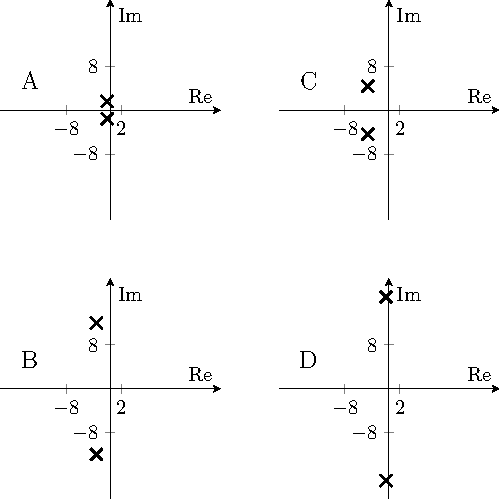
\includegraphics[width=\linewidth]{../../figures/pzmap-apollo}
\end{center}
\end{column}
\begin{column}{0.6\columnwidth}
\begin{center}
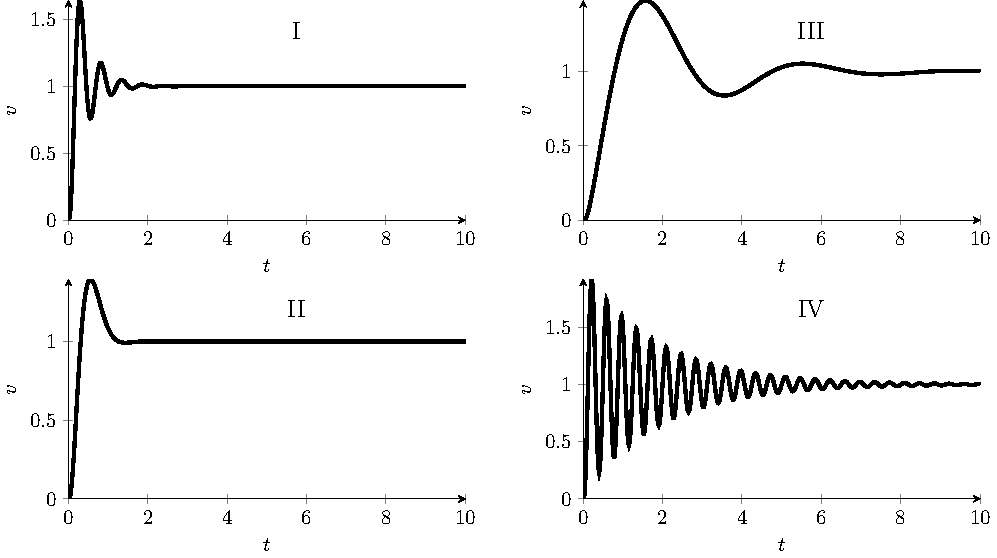
\includegraphics[width=\linewidth]{../../figures/step-response-apollo}
\end{center}
\end{column}
\end{columns}
\end{frame}

\begin{frame}[label={sec:org23ff790}]{Mapping of poles from continuous time to discrete time}
\begin{center}
\begin{tabular}{ll}
Continuous time & Discrete time\\
\hline
\(Y(s) \triangleq \laplace{y(t)}\) & \(Y(z) \triangleq \ztrf{y(kh)}\)\\
\(Y(s) = G(s)U(s) = \frac{b}{s+a}U(s)\) & \(Y(z) = H(z)U(z) = \frac{\beta}{z+\alpha}U(z)\)\\
Pole of the system: \(s+a=0 \; \Rightarrow \; s = -a\) & Pole of the system: \(z+\alpha = 0 \; \Rightarrow \; z = -\alpha\)\\
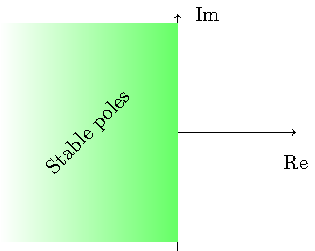
\includegraphics[width=0.22\linewidth]{../../figures/cont-stable} & 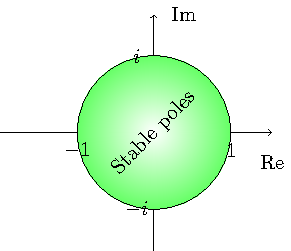
\includegraphics[width=0.22\linewidth]{../../figures/discrete-stable}\\
\hline
\end{tabular}
\end{center}

The \alert{s-domain} of continuous-time systems is related to the \alert{z-domain} of discrete-time systems through  \[z = \mathrm{e}^{sh}\]
\end{frame}

\begin{frame}[label={sec:orgda35d5b}]{Poles in continuous- and discrete time}
\begin{center}
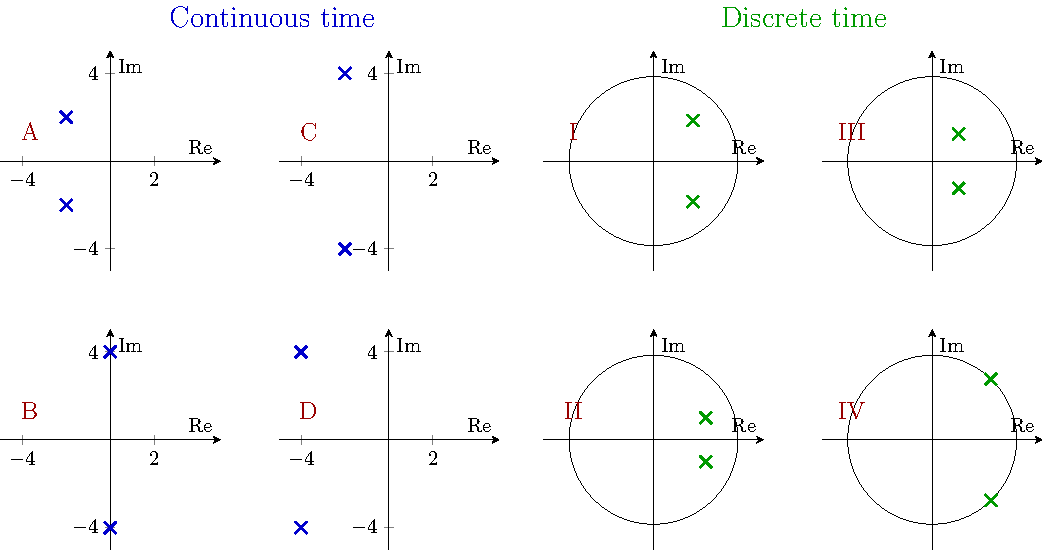
\includegraphics[width=0.85\linewidth]{../../figures/pzmap-continuous-discrete-exc}
\end{center}

\alert{Activity} Pair the continuous-time poles with the corresponding discrete-time poles! \(h=0.2\)
\end{frame}

\begin{frame}[label={sec:org668312d}]{Pole-placement and time-response}
Pair the pole-placement with the correct time-response (discrete time)!
\begin{columns}
\begin{column}{0.4\columnwidth}
\begin{center}
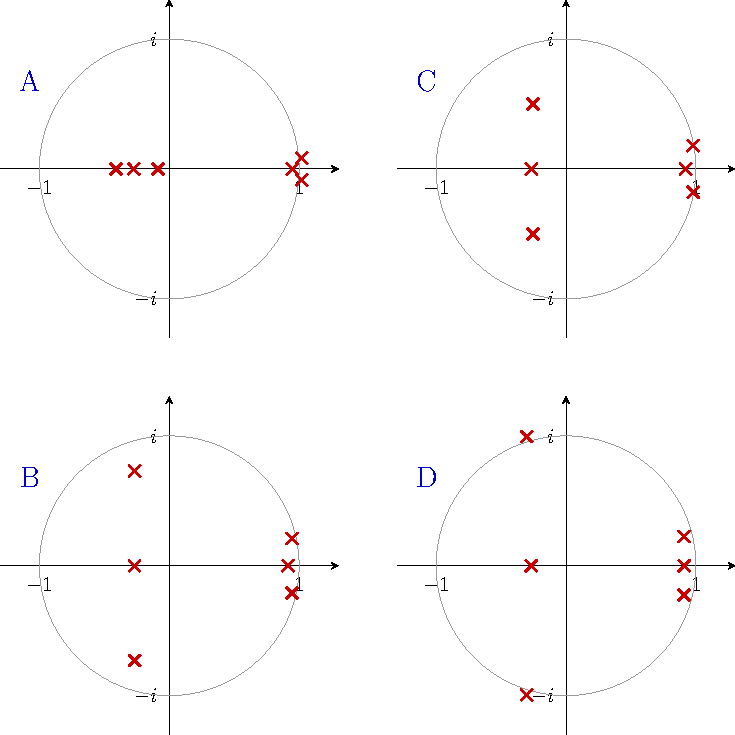
\includegraphics[width=\linewidth]{../../figures/pzmap-discrete-apollo}
\end{center}
\end{column}
\begin{column}{0.6\columnwidth}
\begin{center}
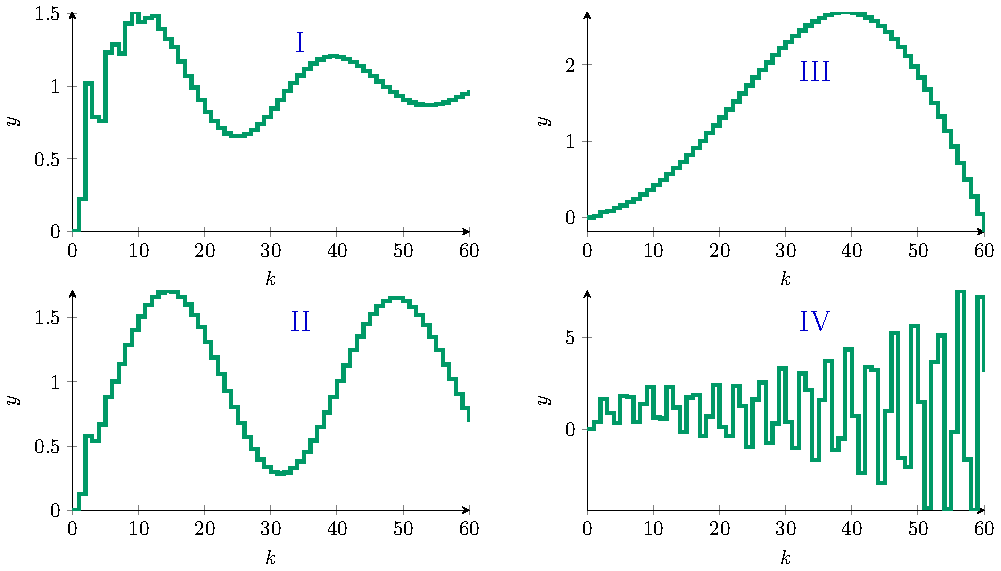
\includegraphics[width=\linewidth]{../../figures/step-reponse-discrete-apollo}
\end{center}
\end{column}
\end{columns}
\end{frame}

\section{Root locus}
\label{sec:org81dea4c}


\begin{frame}[label={sec:orgbc1a858}]{Root locus: A brief review}

\begin{center}
  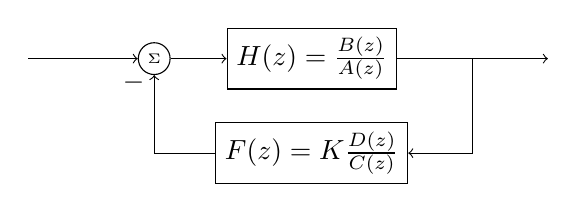
\begin{tikzpicture}[node distance=22mm, block/.style={rectangle, draw, minimum width=15mm}, sumnode/.style={circle, draw, inner sep=2pt}]

    \node[coordinate] (input) {};
    \node[sumnode, right of=input, node distance=16mm] (sum) {\tiny $\Sigma$};
    \node[block, right of=sum, node distance=20mm] (plant)  {$H(z)=\frac{B(z)}{A(z)}$};
    \node[block, below of=plant, node distance=12mm] (controller)  {$F(z)=K\frac{D(z)}{C(z)}$};
    \node[coordinate, right of=plant, node distance=30mm] (output) {};

    \draw[->] (input) -- node[above, pos=0.3] {} (sum);
    \draw[->] (sum) -- node[above] {} (plant);
    \draw[->] (plant) -- node[coordinate] (measure) {} node[above, near end] {} (output);
    \draw[->] (measure) |- (controller);
    \draw[->] (controller) -| node[left, pos=0.95] {$-$}(sum);
  \end{tikzpicture}
\end{center}

\pause


\begin{itemize}
\item The loop pulse-transfer function (loop gain) becomes \(L(z) = H(z)F(z) = K\frac{\overbrace{B(z)D(z)}^{Q(z)}}{\underbrace{A(z)C(z)}_{P(z)}} = K \frac{Q(z)}{P(z)}\).
\end{itemize}
\pause
\begin{itemize}
\item The roots of \(Q(z)\) are called the \alert{open loop zeros}.
\end{itemize}
\pause
\begin{itemize}
\item The roots of \(P(z)\) are called the \alert{open loop poles}.
\end{itemize}
\pause
\begin{itemize}
\item The characteristic equation for the closed-loop system is \[ 1 + K\frac{Q(z)}{P(z)} = 0 \quad \Leftrightarrow \quad P(z) + KQ(z) = 0\]
\end{itemize}
\end{frame}


\begin{frame}[label={sec:orgdddade7}]{Root locus: Definition}
Let
\[\begin{cases} P(z)&=z^n+a_1z^{n-1}+\dots+a_n = (z-p_1)(z-p_2)\cdots(z-p_n)\\ 
Q(z)&=z^m+b_1 z^{m-1}+\dots+b_m=(s-q_1)(z-q_2)\cdots(z-q_m) \end{cases},\ \ \ n\ge m \]

\pause
The root locus shows how the \alert{solution} to the characteristic equation
\begin{equation}
\label{eq:P(z)+KQ(z)=0}
P(z)+K\cdot Q(z)=0,\ \ \ 0\le K<\infty
\end{equation}
depend on the parameter \(K\). The root locus consists of the set of all points in the complex plane that are solutions to \eqref{eq:P(z)+KQ(z)=0} for some non-negative value of \(K\).
\end{frame}

\begin{frame}[label={sec:org0f8aa4c}]{Root locus: Characteristics}
\begin{description}
\item[{Start points}] The \(n\) roots of \(P(z)\), marked by crosses
\item[{End points}] The \(m\) roots of \(Q(z)\), marked  by circles
\item[{Asymptotes}] Number equal to the \emph{pole excess} \(n-m\)
\item[{Real axis}] Some segments of the real axis belong to the root locus
\end{description}
\end{frame}

\begin{frame}[label={sec:org2402d6c}]{Root locus: Direction of the asymptotes}
The characteristic equation \(P(z)+K Q(z)=0\) can be written \(\frac{P(z)}{Q(z)} = -K\) and for large \(z\) it can be approximated as 
\[ \frac{z^n}{z^m} = -K \quad \Leftrightarrow \quad z^{n-m} = -K.\]

Taking the argument of both sides of the equation gives 
\((n-m)\arg z = \pi + k2\pi, \; k \in  \mathbb{Z}\)
So, the \alert{directions} of the asymptotes are given by the expression
\[ \theta_k = \arg z = \frac{(2k+1)\pi}{n-m}, \; k \in \mathbb{Z} \]
\end{frame}

\begin{frame}[label={sec:org7867159}]{Root locus: The asymptotes' intersection with the real axis}
\[ z_{ip} = \frac{ \sum_{i=0}^n p_i - \sum_{i=0}^m q_i}{n-m}, \]
where \(\{p_i\}\) are the starting points (open-loop poles) and \(\{q_i\}\) are the end points (open-loop zeros). 
\end{frame}

\begin{frame}[label={sec:org503865e}]{Root locus exerise: Pair the pulse-trf fcn and root locus}
\begin{columns}
\begin{column}{0.35\columnwidth}
 \small
\begin{align*}
  G_1(z) &= K\frac{(z+2.9)(z+0.2)}{(z-1)^2(z-0.3)}\\[3mm]
  G_2(z) &= K\frac{(z-0.5)(z+0.4)}{(z-1)(z-0.3)(z-0.1)}\\[3mm]
  G_3(z) &= K\frac{(z-0.5)(z+0.8)}{(z-1)^2(z-0.3)}\\[3mm]
  G_4(z) &= K \frac{z-0.6}{(z-1)(z-0.3)}
\end{align*}
\end{column}

\begin{column}{0.65\columnwidth}
\begin{center}
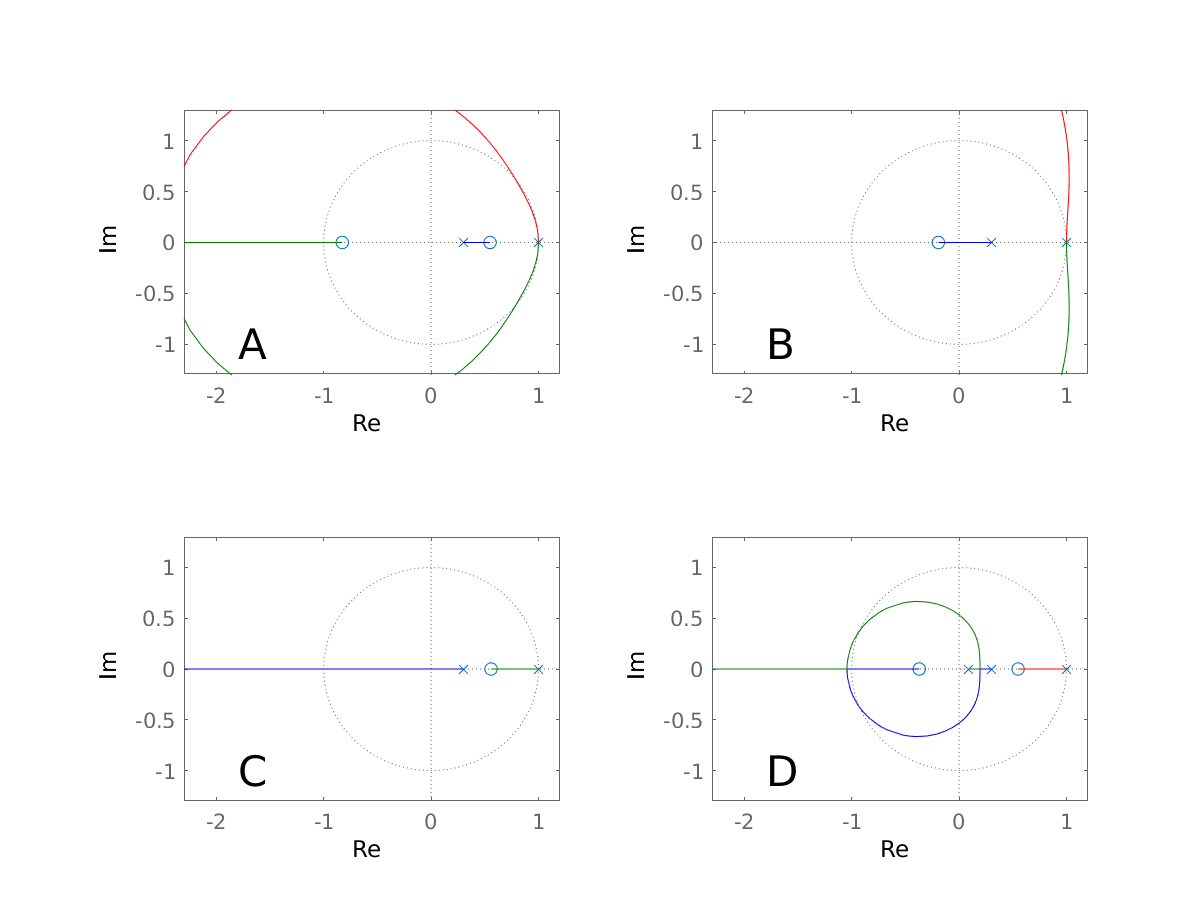
\includegraphics[width=1.04\linewidth]{../../matlab/rlocus_2x2-crop}
\end{center}
\end{column}
\end{columns}
\end{frame}
\end{document}